\documentclass[12pt]{article}
\usepackage{dsfont}
\usepackage{cite}
\usepackage{amsmath}
\usepackage{amsfonts}
\usepackage{mathbbol}
\usepackage{graphicx}
\usepackage{float}
\usepackage{hyperref}
\usepackage{listings}
\begin{document}
\title{Coffee Cooling Challenge \#3: This Time It's Personal}
\author{Daniel Huantes}
\twocolumn
\maketitle
\section{Introduction}
In this final Coffee Cooling Challenge submission I added terms of the differential form of Newton's law of cooling, in order to create a coupled differential equation that represents the cooling of a cup of coffee due to both the heat lost to the air above the liquid, and the sides of the cups surrounding it. The equation I used to model the rate of change in the coffee's temperature, $T$, with respect to time was 
\begin{equation}
\frac{\mathrm{d} T}{\mathrm{d} t} = r_{env} (T_{env} - T) + r_{c} (T_{mug} - T)
\end{equation}
with $T_{mug}$ being the temperature of the mug, changing with time, $T_{env}$ being the temperature of the environment, assumed to be constant over time. We assumed that the room holding the coffee-mug system was large enough that any heat disappated in it would have a negligible effect on it's total temperature. I modeled $\frac{\mathrm{d} T_{mug}}{t}$, the rate of change of the temperature of the mug using
\begin{equation}
\frac{\mathrm{d} T_{mug}}{\mathrm{d} t} = r_{c} (T - T_{mug}) + r_{ce} (T_{env} - T_{mug})
\end{equation}

Unlike our previous challenges, this version of the coffee cooling problem was more difficult as it involed a coupled differential equation, with both $T$ and $T_{mug}$ varying with time, and affecting each other. Another extra challenge added was the ability for the program to handle a variable volume of coffee entered in a more familiar unit (oz), as well as using measurements of a coffee cup I own in order to provide more reliable estimates of the cooling. Both of these issues improve upon the accuracy of the previous problem by introducing more real life factors that affect cooling, and the utility of the program, with being able to model different cups and volumes of coffee.
\section{Discussion}
My initial challenge in creating this version of the Coffee Cooling Challenge was creating a program that could take a variable volume of coffee V and with the physical parameters of the mug holding the coffee, could find the necessary volumes and areas required to calculate the 3 r coefficients in Newton's Law of Cooling I used. I was going to use a truncated cone
\footnote{Actually a right circular frustum of a cone}
in order to model the geometry of a coffee mug such as my own, which although almost cylindrical, like many cups has a mouth wider than its base. My overall goal was to be able to develop a function in order to find the surface area of coffee in contact with the mug, it makes sense that every distinct volume of coffee that the cup could hold would generate it's own unique height and surface radius, however because of the nature of a cone's geometry, solving for any linear portion from a volume leads to a cubic function. Although the function only has a single meaningful root for our purposes, finding a 1 dimensional quantity, to be used as a linking point, from the surface area of the shape is also a quadratic. Then Patrick Cook heard of my struggles to find this equation, and over the weekend distracted himself from GRE prep with my puzzle, and solved it for me. The full solution is most easily represented in 3 equations, here with full credit and thanks to Patrick Cook, who answered my call: ``Patrick, if you figure this out over the weekend don't tell me, I'm trying to work it out on my own''

\begin{equation}
\begin{aligned}
h &= \frac{\mathbb{H}}{\frac{\mathbb{R}}{\mathbb{r}} - 1} \\
R &= \sqrt[3]{\frac{\mathbb{H}\mathbb{r}^3 - \mathbb{r}v + \mathbb{R}v}{\mathbb{H}}} \\
S_A &= \sqrt{\pi ^2 R^4 + 9(\frac{v + \frac{\pi}{3} \mathbb{r}^2 h}{R})^2} \\
& - \pi \mathbb{r} \sqrt{\mathbb{r}^2 + h^2} + \pi \mathbb{r}^2
\end{aligned}
\end{equation}

\begin{enumerate}
\item[$v$--] Volume of liquid
\item[$h$--] ``Truncation height'' of porion of cone below bottom of cup
\item[$\mathbb{H}$--] Height of mug
\item[$\mathbb{R}$--] Major internal radius of mug
\item[$R$--] Radius of the surface of the liquid
\item[$\mathbb{r}$--] Minor internal radius of mug
\item[$S_A$--] Surface area of liquid in contact with mug
\end{enumerate}

I calculated my r constants using Eq. 2 from the Coffee Cooling handout.

The calculation methods for my r constants involved pouring over multiple online lists of thermal properties in order to find a strong approximation of the material my mug is made of. Early contenders were glass and brick, but glass was diaqualified as from anecdotal evidence, grabbing a hot glass out of the microwave is harder than a hot mug. Brick was disqualified as the main source of coefficients for brick was from engineering websites listing the thermal properties of building materials and I had no way of being able to tell which of the wide range of bricks listed would be most accurate at modeling my coffee cup. Ultimately I ended with porcelain, which I determined to be the best approximation of the ceramic in my mug with no obvious way of determining the actual material of which the mug was made\footnote{see possible future work}. The h term in calculating each r coefficient proved to be the hardest to determine. For $r_{e}$, I used the r coefficient provided in the handout, the convective heat transfer coefficient between coffee (water) and air, 15 $\frac{W}{m^2 K}$. For $r_{c}$ I used the thermal conductivity of porcelain divided by the thickness of my cup, using the conductive heat loss of a pipe as an approximation of the heat loss of my cup due to the nearly identical geomtry involved \cite{ET}. Finally for $r_{ce}$ I used the thermal conductivity of porcelain, multiplied by the surface area of the mug directly outside of the liquid (eliminating the contribution of portions of the mug above the coffee line) and dividing by the entire volume bound by this surface area, in order to reach units of $\frac{W}{m^2 K}$. The r values I developed for this model are all very basic approximations, which reflects later in the accuracy of the model, but there is certain aspects that provide promise for more rigorous development of these constants. 
\section{Code}
\begin{figure}[H]
  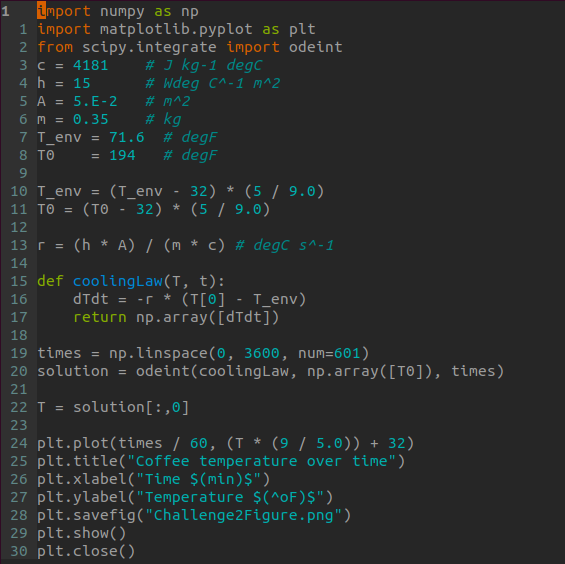
\includegraphics[width=\linewidth]{CodeSnippetCC2.png}
  \caption{My Beautiful Code!}
  \label{fig:mBC}
\end{figure}

\section{Results}
\begin{figure}[H]
  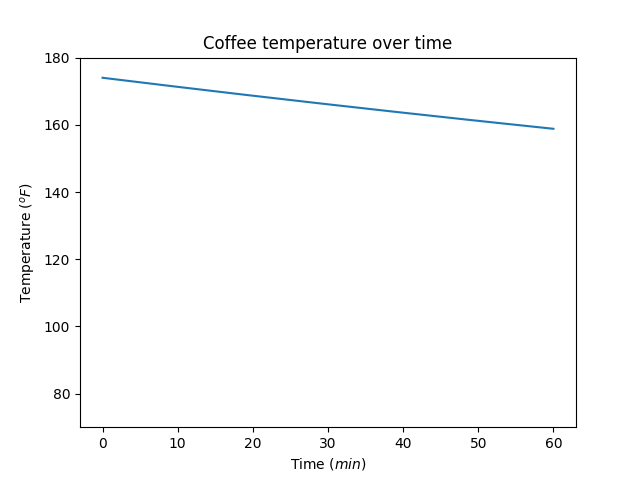
\includegraphics[width=\linewidth]{Challenge2Figure.png}
  \caption{Plot generated from original coffee cooling challenge 2 code, with corrected mass and area}
  \label{fig:plt1}
\end{figure}
 At this point in my work, it became clear that I had reached a natural stopping point, as I was already a week behind from the actual due date of the original coffee cooling problem, and I believe through anecdotal evidence no amount of curve fitting and pouring through lists of thermal coefficients of ceramics will ever get me a date.
\section{Conclusion}
We can tell that numerical methods to solve differentials are an extremely useful tool, because although the analytical solution to this specific function is fairly easily found, it does save us as programmers some work, as well as give us a tool to use in the future for more differentials. In further work, I plan to model thetemperatures of both the liquid inside the coffee and the cup in which it is held, as well as introducing ideas like variable volume of coffee.
\bibliographystyle{unsrt}
\bibliography{references}
\end{document}

